\section{背景} \label{sec:background}


\subsection{Unikernels}

Unikernel は,対象のアプリケーションにリンクし,
アプリケーションと同じ保護モードからのハイパーコールを介して,
下層のハイパーバイザに計算資源を要求する.
Unikernel はリンクされたアプリケーションとアドレス空間を共有するため,
一般的な Unikernel は,マルチプロセスアプリケーションではなく,
シングルプロセスで動作するアプリケーションのみをサポートする.
Unikernel は,特にクラウド環境で受け入れられている.
クラウド環境上の個々の仮想マシン (VM) は通常,
1 つのアプリケーションのみを実行し,
OS の機能の一部のみを使用するためである.
研究者たちは,セキュリティアーキテクチャ~\cite{MadhavapeddyEtAl-Unikernel}や
様々なアプリケーションへのサポート~\cite{KivityEtAl-OSv,ZhangEtAl-Kylinx,WilliamsEtAl-SoCC18,OlivierEtAl-VEE19,KuoEtAl-Lupine},
組み込みクラウド用のマルチテナントコントローラ~\cite{MadhavepeddyEtAl-Jitsu},
軽量ネットワーク機能の仮想化~\cite{MartinsEtAl-NSDI14},
軽量特権仮想マシン~\cite{MehrabEtAl-Kite},
モジュラリティの向上~\cite{KuenzerEtAl-Unikraft,KuenzerEtAl-SYSTOR19},
コンポーネント間の分離の強化~\cite{LefeuvreEtAl-FlexOS,SartakovEtAl-ASPLOS21},
クラウドサービスの軽量化~\cite{GainEtAl-Spacer}
を含む Unikernel の仕組みと適用範囲を研究している.

% \begin{figure}[t]
%     \begin{center}
%       \begin{tabular}{c}
%         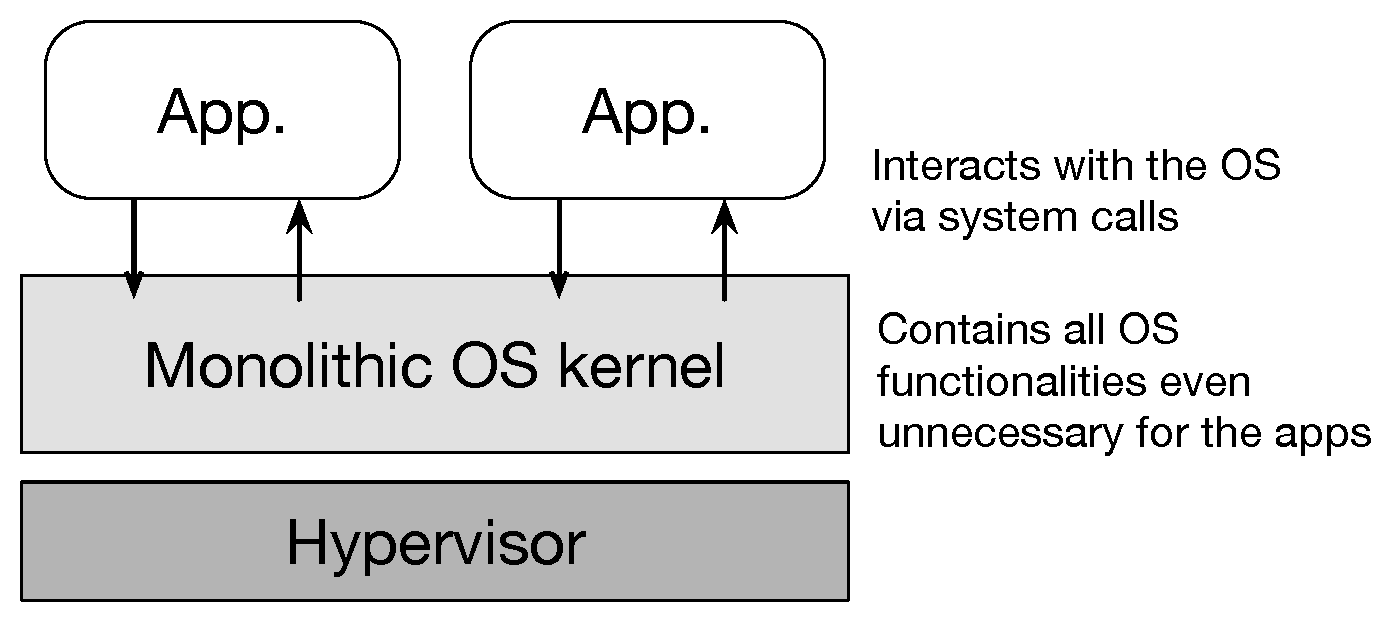
\includegraphics[scale=0.3]{./img/monolithic.eps} \\
%         (a) Conventional Monolithic OS kernel       \vspace*{2mm} \\ 
%         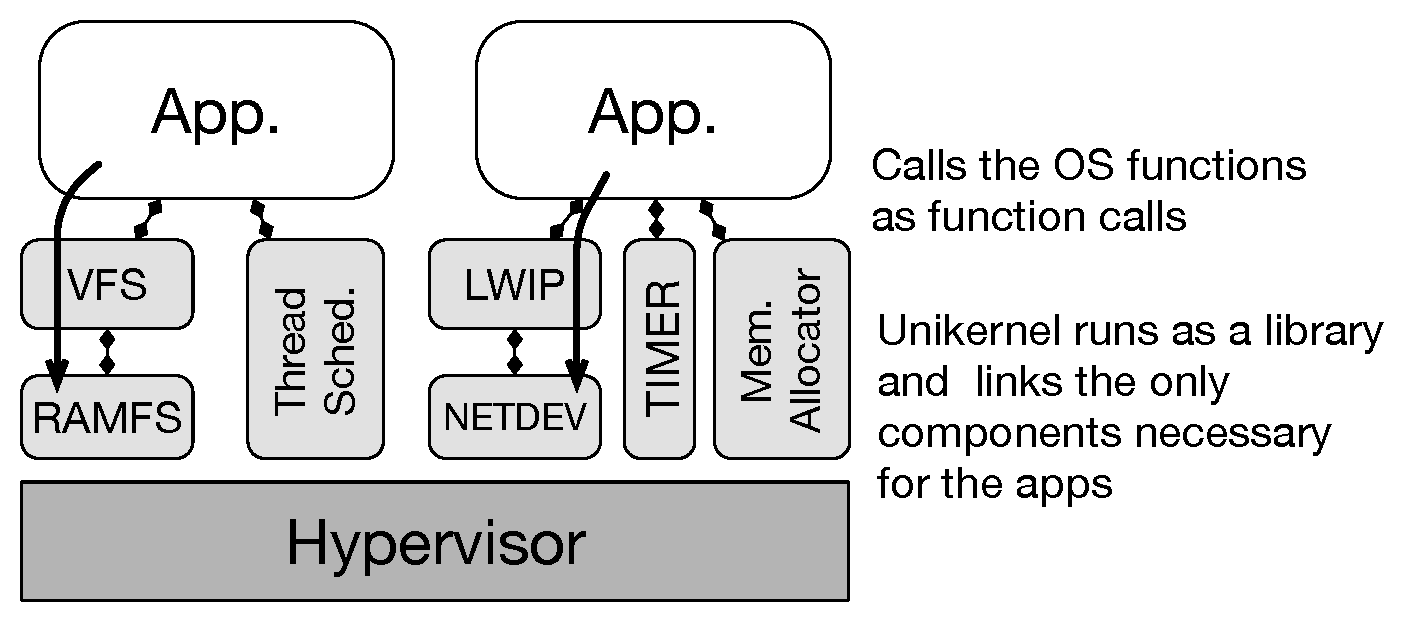
\includegraphics[scale=0.3]{./img/unikernel.eps} \\
%         (b) Unikernel \\
%       \end{tabular}
%       \caption{OS カーネルアーキテクチャの違い}
%       \label{fig:kernels}
%     \end{center}
%   \end{figure}

% 図\ref{fig:kernels}は,従来のモノリシックカーネルと Unikernel の違いを示している.
% Linux のような従来の OS カーネルでは,ファイルシステムやネットワークスタックのようなサブシステムを,その必要性に関係なくすべて含んでおり,
% アプリケーションより高い特権レベルで動作する.
% アプリケーションは計算資源を要求するためにシステムコールを発行し,
% トラップすることによって,下層の OS カーネルに特権的な操作を行わせる.
% 一方で,Unikernel は対象のアプリケーションが動作するのに必要なコンポーネントのみをアプリケーションに直接リンクし,
% 同じアドレス空間で同じ特権モードで動作する.
% アプリケーションは,
% 動作に必要な OS コンポーネントのみを選択して,リンクすることができる.
% これらの特徴は,従来の OS カーネルと比較して,
% 高速なシステムコール発行やブート時間の短縮,
% メモリフットプリントの縮小,OS カーネルレイヤのコードサイズの縮小を含む
% いくつかの利点を提供する.

本論文は,
\emph{どのように Unikernel レイヤのみの効率的な \rr を実現するのか?}
という問いについて答えようとするものである.
Unikernel レイヤの信頼性をできるだけ高いものにしたほうが良い.
Unikernel はアプリケーションとハイパーバイザの中間に位置し,
計算資源をハイパーバイザに要求し,
リンクしたアプリケーションにその計算資源を与えるので,
Unikernel レイヤに障害が発生すると
アプリケーションは実行状態を維持することができなくなるためである.
OS カーネルは,その複雑性と変化し続ける機能から,
過去数十年に渡る多くの努力~\cite{ChouEtAl-SOSP01,PalixEtAl-ASPLOS11,Syzkaller,PanEtAl-SEC17,PailoorEtAl-SEC18,SchumiloEtAl-kAFL, TalebiEtAl-SEC21}
を以ってしてもバグのないソフトウェアからは程遠く,
Unikernel でも同様に,いくつものバグが報告されている\cite{Issues-Unikraft,Issues-OSv,Issues-Mirage}.
報告されているバグの中にはメモリリークといった経年劣化に関連するバグも存在する~\cite{Memleak-Unikraft,Memleak-Mirage}.
また,アプリケーションに必要な機能を提供するために,
アプリケーションの要件に合わせて,
サードパーティ製のライブラリを組み合わせた構成にカスタマイズすることもある.
そのため,Unikernel を定期的に再起動し,
リフレッシュしたメモリの内容の使用させることは,
クラウドサービスを安定して提供するのに有効である.

しかし,効率的な Unikernel の \rr は容易ではない.
Unikernel がアプリケーションと密接に結びつくために,
Unikernel の再起動がアプリケーションの再起動を伴うことになり,
Unikernel に関係のないメモリの内容を消去し,再構築してしまう.
これは,
最近のインメモリデータベースやインメモリ分散フレームワークのようなインメモリアプリケーションにおいて重要なことである.
メモリフットプリントが数十 GB から数百 GB になり,
実行状態の復元に時間がかかるためである.
ある研究では,
Facebook のサーバを一度に 2 \% だけを再起動すると,
再起動時間は約 12 時間まで延長され,
ユーザはクエリの結果の一部しか見ることができないことが報告されている~\cite{GoelEtAl-SIGMOD14}.

% \subsection{\rr}

% 長期稼働するソフトウェアは,
% メモリリークといったソフトウェアバグに起因する
% ソフトウェアの経年劣化(ソフトウェア・エージング)により,
% ソフトウェアの性能が低下し,最終的にはクラッシュやハングアップを引き起こす.

% また,予期せぬフェイラによりクラッシュやハングアップが発生した場合,

% \rr はソフトウェア・エージングを解消しつつ,
% クラッシュやハングアップからのリカバリを可能にするシンプルかつ強力な方法であり,
% ソフトウェアを再起動することでその実行状態を安定させる.
% \rr とは,ソフトウェア若化のプロアクティブな再起動と
% クラッシュやハングアップからのリカバリのためのリアクティブな再起動を合わせたもののことである.
% ソフトウェア若化では,


% ソフトウェアの再起動は,ソフトウェアの経年劣化現象を解消することで未然にクラッシュやハングアップ


% 前者は,定期的なアプリケーションの再起動は,ソフトウェア若化~\cite{HuangEtAl-rejuvenation,CotroneoEtAl-rejuvenation-survey,CotroneoEtAl-Surv14}と呼ばれ,
% 解放忘れのメモリオブジェクトや閉じ忘れのディスクリプタなどのリソースを回収することで,
% ソフトウェアの性能低下やクラッシュ,ハングアップを未然に防ぐことができる.

% ソフトウェアの性能低下やクラッシュ,ハングアップを未然に防ぐことができる.


\subsection{フォルトモデル}

% 本研究では,マイクロカーネルのサーバ単位の再起動~\cite{BhatEtAl-OSIRIS,bLiEtAl-TxIPC}

本研究では,
Unikernel の起動直後の状態をフレッシュな状態と考えており,
その状態に復元することでソフトウェアの動作を安定させる.
そのため,コンパイラやブートコードを TCB に含め,
起動後に動作するコンポーネントで発生するフォルトを対象とする.
また,ハードウェアインフラやハイパーバイザといった Unikernel の下層で動作するソフトウェアを信頼する.

\rr が対象とするフォルトは,大きく二種類に分けることができる.
フォルトが即座にクラッシュを引き起こすようなフェイルストップフォルトと
直接的にクラッシュを引き起こさないものの
ソフトウェアの状態を次第に劣化させるようなフォルトである.
たとえば,ゼロ除算や NULL ポインタ参照などが前者のフェイルストップフォルトであり,
メモリリークやディスクリプタリークなどが後者のソフトウェアの経年劣化現象を引き起こすフォルトである.
\rr ではリアクティブに再起動することでフェイルストップフォルトによるクラッシュからリカバリし,
プロアクティブに再起動することでソフトウェアの経年劣化現象を解消する.

本研究では,Unikernel コンポーネント間のエラー伝搬の防止にも取り組んでいる.
Unikernel はモノリシックカーネルよりもコンポーネントのモジュラリティが高いものの,
アドレス空間や特権レベルなどの分離がなく,すべてのコンポーネント間でエラーが伝搬する可能性がある.
たとえば,既にフォルトが発生して不安定な状態にあるファイルに関係しないコンポーネントが,
仮想ファイルシステム (VFS) コンポーネント内のファイル構造体のオフセットを不正に更新することで,
それ以降のファイル操作が失敗するようになる.
本研究が対象とするコンポーネント間のエラー伝搬とは,分離強度の高い Unikernel である
CubicleOS~\cite{SartakovEtAl-ASPLOS21}や FlexOS~\cite{LefeuvreEtAl-FlexOS} と同じものである.
それらは,あるコンポーネント内のデータに関係ない別のコンポーネントによって,
そのデータが不正に更新されるようなケースを想定している.



% 解放忘れのメモリオブジェクトや閉じ忘れのディスクリプタなどのリソースを回収することで,
% ソフトウェアの性能低下やクラッシュ,ハングアップを未然に防ぐことができる.

% また,Unikernel がリンクするアプリケーションとすべての Unikernel コンポーネントが同じ特権モードで動作し,
% MPK の制御下にあるため,
% 特権モードの違いに起因するエラー伝搬~\cite{ConnorEtAl-PKUPitfalls,VoulimeneasEtAl-CERBERUS,SchrammelEtAl-Jenny}
% が発生することもない.


% \sysname は CubicleOS~\cite{SartakovEtAl-ASPLOS21}や FlexOS~\cite{LefeuvreEtAl-FlexOS}と同じ高い強度で分離を実現するものであるものの,
% このメカニズムで防ぐことができないエラー伝搬が存在する.
% そのエラー伝搬は,
% 関数呼び出し先のコンポーネントのエラーが関数呼び出し元のコンポーネントへと伝搬するケースである.
% このケースは,正当な制御フローの範囲内にバグが存在するときに発生するものであり,
% 関数実行中のコンポーネントが呼び出し元のコンポーネントのデータを不当に更新することである.

% このケースのエラー伝搬を完全に防ぐためには,
% 他のコンポーネントのデータ更新時の正当性を関数ごとに検証する必要がある.
% しかし,Unikernel はリンクするアプリケーションの要件によって,
% コンポーネントの構成が異なるため,
% 同じ関数であっても,関数の呼び出し元と呼び出し先のコンポーネントの関係が一定であるとは限らず,
% データ更新の正当性を定義することが難しい.


\subsection{過去のアプローチ}

いくつかのアプローチは Unikernel の信頼性の向上を目的としている.
Unikraft~\cite{KuenzerEtAl-Unikraft}は,
Unikernel のモジュラリティを高め,
TCB をできるだけ小さくすることによってカスタマイズ性と信頼性を向上させている.
CubicleOS~\cite{SartakovEtAl-ASPLOS21}と FlexOS~\cite{LefeuvreEtAl-FlexOS}は,
フォルトしたコンポーネントから他のコンポーネントへのエラー伝搬を防ぐために
Unikernel のコンポーネント同士を強く分離するものである.
これらのアプローチは,
アプリケーションのコンポーネントやサードパーティ製のライブラリなどからの
悪意のある攻撃から Unikernel の機密性と完全性を保護することを目的とするものである.
これらのアプローチでは,Unikernel が経年劣化に関連したバグに悩まされることがないことを保証できないのに対し,
私たちのアプローチでは Unikernel を \rr することでその悪影響を軽減することができる.


対象のソフトウェアを効率的に再起動するための
ソフトウェアメカニズムはこれまでにも模索されている.
いくつかの研究では OS カーネルの効率的な再起動に注目している.
KUP~\cite{KashyapEtAl-KUP}は,OS カーネルが再起動しても,アプリケーションの実行を維持する.
KUP は,メモリ上の対象のアプリケーションのユーザスペースのチェックポイントメカニズム~\cite{CRIU}を用いたスナップショットを取得し,
OS の再起動後にスナップショットを復元する.
このアプローチを Unikernel にリンクされたアプリケーションに適用することはできない.
従来の OS カーネルとは異なり,
リンクされたアプリケーションと共有する単一のアドレス空間のみをサポートする Unikernel では,
チェックポイントの取得処理を対象のアプリケーションと同時に実行することができない.
また,
アプリケーションと Unikernel の境界が不明確であり,Unikernel のカスタマイズ性のために通常のアプリケーションとは異なるため,
Unikernel にリンクされたアプリケーション以外が,対象のアプリケーションレイヤのみのスナップショットを取ることは困難である.


Otherworld~\cite{DepoutovitchEtAl-otherworld}や Dwarf~\cite{TeradaEtAl-Dwarf}は,
アプリケーションを動作させながら OS カーネルの再起動をする.
OS カーネルを再起動する際に,
Otherworld は新しいカーネルを起動し,
古い OS カーネルのメモリ上のプロセスコンテキストのカーネルメモリオブジェクトを回収し,
その内部構造を新しい OS カーネルに復元する.
Dwarf は,対象のアプリケーションに対するプロセスコンテキストのコアをハイパーバイザに保存し,
新しく起動した仮想マシン上に OS カーネルを起動し,
対象のアプリケーションを古い仮想マシンから新しい仮想マシンへと移行しながら,
新しいカーネルにアプリケーションの動作状態を復元させる.
これらのアプローチは,対象の OS カーネルが\emph{モノリシック}であるということを前提にしている.
Unikernel の構成がアプリケーションごとに異なり,
プロセスコンテキストを維持するためのカーネルオブジェクトが一定ではないため,
Unikernel の特性に適したアプローチとはいえない.
これらのアプローチを Unikernel に適用するためには,
Unikernel がリンクするアプリケーションごとにメカニズムを再設計する必要があり,
それは簡単な作業ではない.

Microreboot~\cite{CandeaEtAl-Microreboot}は,
細かい粒度でのソフトウェアの再起動を実現する.
Microreboot を可能にするために,
対象のアプリケーションは
再起動の単位となる独立した小さいソフトウェアコンポーネントに分割される.
小さいコンポーネントの再起動がフォルトからリカバリ できない場合には,
より大きいコンポーネントが再起動される.
このアプローチの暗黙の仮定として,
Microreboot される各コンポーネントは状態を持たないので,
対象のアプリケーションは,任意のコンポーネントの再起動に渡って,
継続して動作し続ける.
Unikernel のコンポーネントは状態を持つことが多く,
ファイルシステムやネットワークのような状態を持つコンポーネントの再起動に渡って,
アプリケーションが継続して動作することは難しい.

Phase-based Reboot~\cite{YamakitaEtAl-PBR}や ShadowReboot~\cite{YamadaEtAl-ShadowR},CacheMind~\cite{KouraiEtAl-cachemind}を含む
効率的な OS の再起動に対するアプローチは,
OS カーネルの再起動によって引き起こされるダウンタイムとパフォーマンスの低下を軽減する.
通常の OS の再起動のように,これらのアプローチはすべての動作中のアプリケーションの再起動を伴い,
メモリフットプリントが大きなインメモリアプリケーションにおいて深刻なパフォーマンスの低下を引き起こす.
ハイパーバイザのソフトウェア若化をサポートするアプローチでは,
ハイパーバイザの再起動渡って,仮想マシンの動作状態を維持する.
これらのアプローチは,私たちのアプローチと補完関係にある.

% A. Unikernels
% The unikernel is linked to the target applications and
% requests computational resources to the underlying hypervi-
% sor via hypercalls from the same protection mode as the
% applications. The unikernel shares the address space with
% the linked applications; typical unikernels support single-
% process applications, not multi-process ones. The unikernel
% is accepted especially in cloud platforms because each virtual
% machine on modern cloud platforms typically runs only one
% application and uses only parts of OS functionalities. Re-
% searchers have studied unikernel’s architectures and applica-
% bility including secure architectures [25], supports for various
% applications [16], [28], [36], [39], multi-tenant controller for
% embedded clouds [24], lightweight network function virtual-
% ization [26], lightweight privilege virtual machines [27], im-
% provements of the modularity [20], [21], and the enhancement
% of isolation between components [23], [32].
% Fig. 1 shows the difference between the conventional mono-
% lithic OS kernels and unikernels. The conventional OS kernels
% like Linux contain all subsystems such as file systems, memory
% managers, and network stacks, regardless of the necessity of
% the running applications, and run at a higher privilege level
% than the applications. The applications issue system calls to
% request computational resources and privilege operations to
% underlying OS kernels by causing traps. On the other hand,
% the unikernels are directly linked to the target applications
% and run on the same address spaces and privilege mode. The
% applications can choose and link the only kernel components
% they require to run. These features provide several benefits,
% including faster system call issues and boot time, smaller
% memory footprint, and smaller code of the OS kernel layer
% than conventional OS kernels.
% In this paper, we try to answer the following question: How
% do we rejuvenate unikernels efficiently? It is better to make
% the unikernel layer as reliable as possible. Since unikernels are
% intermediate between applications and hypervisors to request
% computational resources to the hypervisor and give the re-
% sources to the linked applications, the applications cannot keep
% running when their unikernel layers fail. OS kernels are still
% far from bug-free software even with numerous efforts [2], [6],
% [29]–[31], [33], [34] in the past decades due to its complex and
% ever-changing functionalities, and thus, the periodic restarts of
% unikernels to enforce them to use fresh memory contents are
% helpful to offer cloud services stably.
% The efficient rejuvenation of unikernels, however, does not
% come for free. Since the unikernels are tightly coupled with
% the applications, the rejuvenation of the unikernels involves
% restarting the applications, causing the elimination and restora-
% tion of memory contents unrelated to unikernels. This is non-
% trivial for modern in-memory applications such as in-memory
% databases and in-memory distributed frameworks because their
% memory footprints are tens to hundreds of GB of memory and
% restoring running states is time-consuming. A research paper
% reported that restarting only 2% of Facebook’s servers at a
% time prolongs the restart duration to about 12 hours, during
% which time users see only partial query results [10].
% B. Previous Approaches
% Software mechanisms for efficiently rebooting the target
% software have been explored so far. Some work focuses on ef-
% ficient OS kernel reboots. KUP [15] keeps the application run-
% ning across the OS kernel reboots. KUP takes snapshots of the
% target applications in memory with user-space checkpointing
% mechanisms [1], and restores them after the OS reboot. This
% approach is not applicable to unikernel-linked applications.
% Unlike conventional OS kernels, the checkpointing process
% cannot run with the target application on a unikernel that
% supports only a single address space shared with the linked
% application. Also, taking snapshots of the only application
% layers is difficult outside unikernel-linked applications because
% the boundary between applications and unikernels is unclear
% and different from the applications due to the customizability
% of the unikernel.
% Otherworld [9] and Dwarf [35] restart the OS kernels,
% keeping applications running. In restarting the OS kernel,
% Otherworld launches the newer kernel and forces it to salvage
% kernel memory objects of the process contexts in the older
% kernel’s memory and restore its internal structures. Dwarf
% stores the cores of process contexts for the target applications
% to the hypervisor, launches the OS kernel on a newly-launched
% virtual machine, and forces the kernel to restore them while
% migrating the target applications from the old virtual machine
% to the newly-launched one. The assumption behind these
% approaches is that the target OS kernels are monolithic, and
% the approaches are not suitable for the characteristics of the
% unikernels; since the unikernel’s components are different
% between applications, the kernel objects to maintain process
% contexts are not constant. The redesign of these mechanisms
% for each unikernel-linked application is required and a non-
% trivial task.
% Microreboot [5] achieves fine-grained software reboots. To
% enable a microreboot, the target application is divided into
% small independent software components which become units
% for a reboot. If rebooting a small component cannot recover
% from a failure, a bigger component will be rebooted. The
% implicit assumption of this approach is that each component
% to be microrebooted is so stateless that the target applica-
% tions consistently run across some components’ reboots. The
% components of the unikernels are often stateful; thus, it is
% difficult for the linked applications to consistently run across
% rejuvenating stateful components such as file systems and
% networks.
% Approaches for efficient OS reboots, including Phase-based
% reboots [38], ShadowReboot [37], and CacheMind [17] reduce
% downtime and performance degradation incurred by the OS
% kernel reboots. Like regular OS reboots, these approaches
% involve all running applications’ restart and thus cause sig-
% nificant performance degradation for modern in-memory ap-
% plications whose memory footprints are large. Approaches
% to support hypervisor rejuvenation [18], [19], [22] allow us
% to keep running states of the virtual machines across the
% hypervisor rejuvenation. These approaches are complementary
% to ours.
% Some approaches aim at the improvement of the uniker-
% nel reliability. Unikraft [20] enhances the modularity of the
% unikernels to improve their customizability and reliability by
% making their TCB as small as possible. CubicleOS [32] and
% FlexOS [23] strongly isolate unikernel components from each
% other to prevent error propagation from faulted components to
% the other ones. These approaches are complementary to ours to
% attain the reliability of the unikernel-linked applications. Since
% these approaches do not guarantee that the unikernels never
% suffer from aging-related bugs, our approach can mitigate their
% adverse effects by making the unikernels rejuvenatable.